\documentclass[times, utf8, seminar, numeric]{fer}
\usepackage{booktabs}
 \usepackage{url}

\begin{document}

% Ukljuci literaturu u seminar
\nocite{*}

% TODO: Navedite naslov rada.
\title{Faza konsenzusa u OLC paradigmi sastavljanja genoma – Sparc}

% TODO: Navedite vaše ime i prezime.
\author{Nikola Bukovac, Vinko Kolobara}

% TODO: Navedite ime i prezime voditelja.
\voditelj{Mile Šikić}

\maketitle

\tableofcontents

\chapter{Uvod}
Uvod...

\chapter{Sparc algoritam}
Algoritam Sparc je algoritam faze konsenzusa u Preklapanje-Razmještanje-Konzenzus (engl. \emph{Overlap-Layout-Consensus, OLC}) pristupu sastavljanja očitanja genoma. Kao temelj algoritma se koristi de Bruijn/k-mer graf nad kojim se potom provodi ostatak algoritma (Sparc referenca).
\section{Opis algoritma}
Prvi korak algoritma je konstrukcija k-mer grafa na temelju predanog ulaza koji sadrži izlaz iz faze Razmještaja, OLC metode. Ovisno o parametrima \emph{k} i \emph{g} kreira se inicijalni k-mer graf, gdje navedeni parametri određuju strukturu grafa, konkretno \emph{k} specificira koliko će nukleotida biti sadržano u pojedinom čvoru grafa, a \emph{g} specificira koliko će se nukleotida nalaziti na svakom bridu. Inicijalni graf je usmjeren sa samo jednim bridom iz svakog vrha osim zavšnog, koji ga nema. Razlika između ovog grafa i klasičnog de Bruijn grafa je u to tome što su isti k-meri na različitim pozicijama nezavisni jedni od drugih dok su kod de Bruijn grafa smješteni u jednom vrhu pa se ovaj graf smatra \emph {sparse} grafom. Sljedeći korak algoritma je poravnjanje dodatnih slijedova čiji se postupak se provodi ovisno o tome da li k-mer u novom slijedu odgovara k-meru u originalnom slijedu i njegovom bridu gdje se onda samo poveća težina brida za definiranu težinu ili ukoliko ne odgovara dodaje se novi brid u graf i kreira se dodatni k-mer i samim time kreira se novi put u grafu. Ovaj postupak je jako sličan kreiranju de Bruijn grafa, ali zbog razlikovanja istih k-mera ovisno p njihovoj poziciji, postoji razlika u postupku. Ovaj korak se ponavlja za sve slijedove koje smo dobili sekvenciranjem. Završni korak Sparc algoritma je traženje puta u grafu koji ima najveću težinu, što je zahvaljujući činjenici da je konstruirani graf usmjeren i acikličan moguće napraviti s BFS ili DFS algoritmom kojim računamo težinu svakog vrha u grafu. Rekonstrukcija slijeda se provodi tako da krenemo od najtežeg vrha i vraćamo se po najvećim težinama natrag sve do početnog vrha. Kompleksnost algoritma...

\section{Primjer}
\begin{figure}[htb]
	\centering
	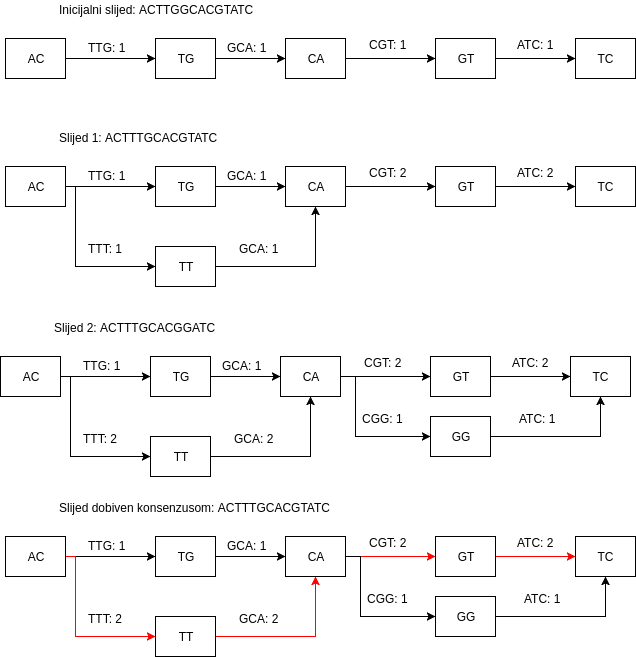
\includegraphics[scale=0.6]{images/backbone.png}
	\caption{Postupak izgradnje grafa s k=2, g=3}
	\label{example}
\end{figure}

Na gornjoj slici je prikazan cjelokupni postupak algoritma Sparc. Inicijalni slijed služi za kreiranje inicijalnog lanca (engl. \emph{backbone}). Nakon kreiranja \emph{backbone}-a grafa, sljedeći slijed poravnavamo tako da krećemo od početka slijeda i vidimo da je prvi k-mer AC jednak k-meru kontruiranom u grafu, ali je prijelaz na sljedeći k-mer TTT različith od onoga koji se već nalazi u grafu te je stoga potrebno konstruirati novi k-mer TT te novi brid iz k-mera AC prema novom k-meru TT, a taj brid je TTT. Slijedećih g nukleotida je GCA koji trebaju završiti u k-meru CA koji već postoji u konstruiranom grafu te je potrbno kreirati brid CGA od k-mera TT prema k-meru CA. Sljedećih g nukleotida je CGT, budući da taj brid postoji u konstruiranom grafu potrebno je samo povećati težinu postojećeh brida, isto vrijedi i za sljedećih g nukleotida ATC. Postupak je jednak i za slijed 2. Za određivanje najtežeg puta pratimo bridove s najvećim težinama, a u ovdje kontruiranom grafu to je put od k-mera AC bridom TTT potom bridom GCA, CGT i ATC te je stoga rekonstruirani slijed ACTTTGCACGTATC.

\chapter{Naša implementacija algoritma}
Uvodna nora
\section{Korišteni formati}

\subsection{FASTA}
Naš algoritam ovaj format koristi kako bi napravio početni slijed(engl. backbone) za ulaz te na izlaz stavlja rekonstruirani slijed također u FASTA formatu.
Ulaz u naš algoritam je u biti izlaz iz faze razmještaja OLC metode.
\subsection{FASTQ}
Sličan FASTA formatu, ali osim samog slijeda sadrži i oznaku kvalitete svakog očitanja.
Ovaj format podataka sadrži sekvencirane slijedove koji će poslužiti za rekonstrukciju originalnog slijeda.
Iako naša implementacija ne koristi direktno ovaj format podataka, on se koristi kao ulaz za alat graphmap koji služi za generiranje SAM formata podataka.
\subsection{SAM}
Ovaj format podataka sadrži grupirane informacije o svim očitanjima iz FASTQ formata podataka. Podaci iz ovog formata podataka služe za rekonstrukciju genoma. Popis korištenih podataka...
\section{Korištene biblioteke}
C++ STl i graphmap
\subsection{Graphmap}
Malo o graphmap biblioteki
\section{Struktura implementacije}
Pregled napravljenog rješenja
\section{Instalacija i pokretanje algoritma}
Objašnjenje kako se implementacija instalira i pokreće

\chapter{Analiza implementacije}
Za utvrđivanje uspješnosti kvalitete implementacije, radimo usporedbu slijeda koji smo koristili kao ulaz u algoritam te slijeda koji smo dobili kao izlaz iz algoritma što radimo tako što oba slijeda uspoređujemo sa referentnim slijedom koji nam služi za određivanje koliki je postotak podudarnosti ulaznog i izlaznog slijeda s referentnim. Postotak podudarnosti slijedova nam je najbitniji podatak prilikom analize, ali jednako tako su nam važni i podaci o utrošku memorijskog prostora te vremenu izvođenja algoritma.
\section{Alati za analizu}
Kako bi analiza podataka bila što preciznija koristimo gotove alate, kojima provjeravamo prije navedene čimbenike koje pratimo.
\subsection{DnaDiff}
DnaDiff je alata iz programskog paketa mummer ...
\subsection{cgmemtime}
\section{Testna konfiguracija}
Detalji o računalima na kojima se vršila analiza
\section{Analiza utroška memorije}
Analiza i usporedba memorije za naš i referentni algoritam
\section{Analiza utroška vremena}
Analiza i usporedba vremena za naš i referentni algoritam

\chapter{Zaključak}
Zaključak.

\bibliography{literatura}
\bibliographystyle{fer}

\chapter{Sažetak}
Sažetak.

\end{document}
